\documentclass{article}
\usepackage{amsmath}
\usepackage{tikz}
\usetikzlibrary{arrows.meta}

\begin{document}

\begin{figure}[h]
    \centering
    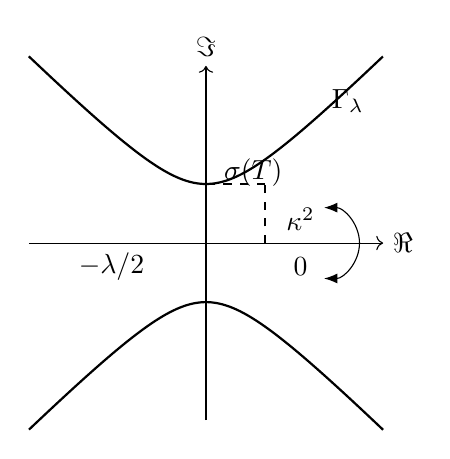
\begin{tikzpicture}[scale=1.5]
        % Axes
        \draw[->] (-1.5,0) -- (1.5,0) node[right] {$\Re$};
        \draw[->] (0,-1.5) -- (0,1.5) node[above] {$\Im$};
        
        % Contour
        \draw[thick, domain=-1.5:1.5, variable=\x, samples=100]
            plot ({\x}, {sqrt(\x*\x + 0.25)});
        \draw[thick, domain=1.5:-1.5, variable=\x, samples=100]
            plot ({\x}, {-sqrt(\x*\x + 0.25)});
        
        % Labels
        \node at (1.2, 1.2) {$\Gamma_\lambda$};
        \node at (-0.8, -0.2) {$-\lambda/2$};
        \node at (0.8, -0.2) {$0$};
        \node at (0.8, 0.2) {$\kappa^2$};
        \node at (0.4, 0.6) {$\sigma(T)$};
        
        % Dashed line
        \draw[dashed] (0, 0) -- (0.5, 0);
        \draw[dashed] (0.5, 0) -- (0.5, 0.5);
        \draw[dashed] (0.5, 0.5) -- (0, 0.5);
        \draw[dashed] (0, 0.5) -- (0, 0);
        
        % Arrows
        \draw[-Latex] (1.3, 0) arc (0:90:0.3);
        \draw[-Latex] (1.3, 0) arc (0:-90:0.3);
    \end{tikzpicture}
    \caption{An illustration of the contour $\Gamma_\lambda$ defined in \cref{eq:contour}. The region enclosed by $\Gamma_{\lambda}$ is just $D_\lambda$ in \cref{assu:Filter}. The dashed interval $[0,\kappa^2]$ contains the spectrum of $T$ and $T_X$.}
    \label{fig:contour}
\end{figure}

\end{document}